\documentclass{article}
\usepackage[backend=biber]{biblatex}
\usepackage{tikz}
\usetikzlibrary{positioning}
\usepackage{float}
\usepackage{amsmath}
\usepackage{enumitem}
\usepackage{gensymb}
\usepackage{pgfplots}
\usepackage{csvsimple}
\usepackage{filecontents}
\usepackage{multirow}
\usepackage{graphicx}
\usetikzlibrary{calc,arrows,positioning}

\definecolor{dkgreen}{rgb}{0,0.6,0}
\definecolor{gray}{rgb}{0.5,0.5,0.5}
\definecolor{mauve}{rgb}{0.58,0,0.82}

\addbibresource{references.bib}

\newcommand{\tablerow}[4]{ #1 & #2 & #3 & #4\\}
\newcommand{\n}[0]{\\[\baselineskip]}

\title{CS3105 Learning Noughts and Crosses}
\date{2017-04-12}
\author{140011146}

\begin{document}

\maketitle

\pagenumbering{arabic}


\section{Introduction}
In this practical we were asked to create a multi-layer feed-forward neural network that is trained to play Noughts and Crosses (or Tic-Tac-Toe) and provide the relevant datasets.

I was successful in creating a neural network with error back propagation in Python. To train the network to play the game, I first trained it to play against a random AI...
\section{Implementation of neural net}
My implementation was written in Python. I chose to use Python because \texttt{numpy} was a very useful library for matrix and vector multiplication, allow me to calculate outputs/errors of each layer very simply. 


\section{Design of network}
\subsection{Initial weights and biases}
I first initialise the weights and biases of the network using a random Gaussian distribution of mean 0 and variance 1 (\texttt{np.random.randn}). However, this is obviously not optimal as the random weights and biases are not accurate and so would take longer to converge to the desired output. 
\n
According to \cite{DBLP}, it is fine to have biases be initialised to zero, but weights must not be initialised to the same value to avoid symmetry in the neurons of the hidden layer.

\subsection{Finding the right design}
I realised soon after initial testing of the network that there was a very large parameter space to experiment with. From the types of activation and cost function of the network, to the learning rate and number of hidden neurons, all these parameters affected the performance of the network and also how quickly it converged.
\subsubsection{Number of hidden neurons}
To experimentally find what number of hidden neurons is a good choice, I run a script, playing and training the neural network after each game. I found that after playing roughly 10000 games, the win rate of the network starts to converge. To reduce variance due to the randomly set weights, I ran each experiment 100 times, varying the size of the hidden layer in each experiment and calculating the average win rate that the network achieved with those parameters. The script I used for these experiments can be found in \texttt{parameters.py}. The script takes a while to run, so I distributed the load, running each experiment on different machines.

\begin{figure}[H] 
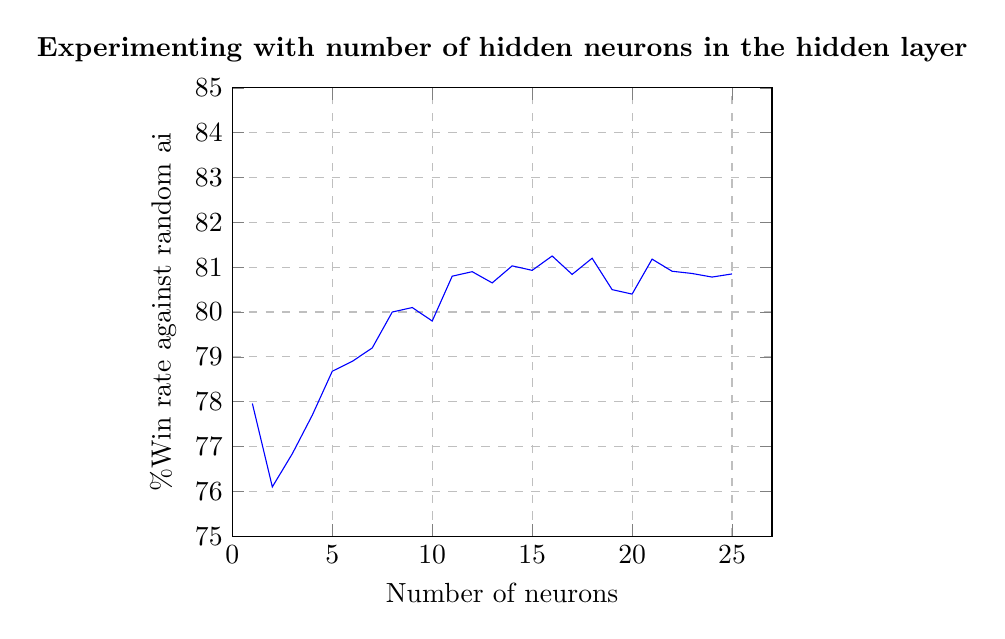
\begin{tikzpicture}
\begin{axis}[
    title={\textbf{Experimenting with number of hidden neurons in the hidden layer}},
    xlabel={Number of neurons},
    ylabel={\%Win rate against random ai},
    xmin=0, xmax=27,
    ymin=75, ymax=85,
    xtick={0,5,10,15,20,25},
    ytick={75, 76, 77, 78, 79, 80, 81, 82, 83, 84, 85},
    legend pos=north west,
    ymajorgrids=true,
    xmajorgrids=true,
    grid style=dashed,
]

\addplot
	[color=blue, mark=circle,]
    coordinates {(1, 77.96) (2, 76.1) (3, 76.84) (4, 77.7) (5, 78.68) (6, 78.9) (7, 79.2) (8, 80) (9, 80.1) (10, 79.8) (11, 80.8) (12, 80.9) (13, 80.65) (14, 81.03) (15, 80.93) (16, 81.25) (17, 80.84) (18, 81.2) (19, 80.5) (20, 80.4) (21, 81.18) (22, 80.91) (23, 80.86) (24, 80.78) (25, 80.85)};
    \label{myftpcmp}
	
\end{axis}
\end{tikzpicture}
\caption{Testing number of hidden neurons with one hidden layer}
\label{1hiddenlayer}
\end{figure}
I noticed while playing around adjusting the parameters of the network that a network with layers (9, 18, 18, 9) seemed to converge to over 80\% win rate very quickly and could even reach win rates of up to 90\% given enough time. According to \cite{faq}, for most general neural network problems, one hidden layer is usually enough. However, I wanted to test with two hidden layers to see if there is any change in performance or if the network would converge faster, or if I had just gotten lucky when trying the (9, 18, 18, 9) network. 
\n
\begin{figure}[H]
\begin{tabular}{ |c|c|c|c|c|c|c|c| }
\hline
\multirow{2}{10.5em}{\textbf{Second hidden layer}} & \multicolumn{7}{c|}{\textbf{First hidden layer}} \\
\cline{2-8}
& \textbf{9} & \textbf{12} & \textbf{15} & \textbf{18} & \textbf{21} & \textbf{24} & \textbf{27} \\
\hline
\textbf{9} & 1497 & 1675 & 1445 & 1614 & 1231 & 1340 & 1769\\
\hline
\textbf{12} & 1339 & 1333 & 1398 & 988 & 1082 & 929 & 946 \\
\hline
\textbf{15} & 1656 & 796 & 942 & 985 & 1033 & 665 & 616\\
\hline
\textbf{18} & 1255 & 645 & 902 & 1009 & 602 & 763 & 714\\
\hline
\textbf{21} & 1393 & 1189 & 991 & 826 & 888 & 588 & 882\\
\hline
\textbf{24} & 787 & 1070 & 955 & 988 & 590 & 557 & 549\\
\hline
\textbf{27} & 943 & 1007 & 841 & 721 & 549 & 1061 & 622 \\
\hline
\end{tabular}
\caption{Testing number of hidden neurons with two hidden layers for the number of games required to converge to a 75\% win rate against a random AI}
\label{2hiddenlayers}
\end{figure}

Figure \ref{2hiddenlayers} shows the results for testing with two hidden layers. Here instead of testing the win rate, I test how many games it takes for the network to reach a 75\% win rate. This is because I wanted to find out if and how the number of hidden layers and neurons affected the speed of convergence. From the table we can see that having more hidden neurons in each layer increases the speed of convergence 



\subsubsection{How to train the network}
Another question was how to train the network. Playing it against a random AI was reasonable since it should develop at least some winning strategy, but should it be trained after every game or every batch of games? Additionally, it could be trained on the wining moveset positively or the losing moveset negatively so it doesn't do those moves again. The draws should also not be dismissed in training, as we know a perfect game results in a draw, so perhaps it should be trained on the drawing moves instead of the winning or losing moves?
\n
To train and winning and drawing games, I take the all the moves that the network made (stored in \texttt{tictictac.history}) and train the network on a small learning rate and epoch over this small set of data. The reason the learning rate and epoch size is small is because the network should not learn too strictly to this small dataset. Thousands of games will be played and each game trained this way, so the network should learn slowly and incrementally over all these games. For testing against a random AI player, I found that the network would win very quickly by going in a straight line, but its strategy was not very smart. This is because the random player very rarely will block the network's winning move, resulting in the network learning the same moves to win every game but not learn about blocking the opponent. This is a good starting point as it has learned to win, but it hasn't learned much outside of that.
\n
An improvement to this is to train the network on loses as well. This attempts to teach the network which moves were bad and works in reverse to how training winning moves works. The last move (the losing move) that the network made is taken and the results inversed (i.e, instead of the output list being [0, 0, 0, 1, 0, 0, 0, 0, 0] where 1 is the position that the network played, the output for training the loss is [1, 1, 1, 0, 1, 1, 1, 1, 1]) to teach the network to try and make a different move instead of the losing one. 
\n
To test this, I ran the same network, training it exclusively on winning, drawing and losing movesets  

\subsection{Final design of neural net}
From my experiments on testing the network parameters, I decided to create the neural network with layers (9, x, 9) for the size of the input, hidden and output layers respectively. I only test with one hidden layer as multiple references have stated than in general, only one hidden layer is required for most problems \cite{faq}.
\section{Testing}
To test that my neural network was implemented correctly, I gave it two training examples and trained it on 1000 epochs. Afterwards, I fed the input of the two examples into the network and checked the output to see if there were close to the expected output. In addition to just checking the values of the output of the network, I also print the value of the cost function after a certain number of epochs. If the value of the cost function is converging to zero, then I know the network is working for those training examples. The script used for this can be found in \texttt{test.py}. 
\section{Evaluation}

\section{Conclusion}



\section{Files in submission}

\printbibliography


\end{document}